\section{Kotlin}\label{chapter:kotlin_multiplatform}

W ramach systematycznego przeglądu literatury (przedstawionego w Rozdziale \ref{chapter:przeglad_literatury}) zauważono, że aktualne badania skupiają się wyłącznie na języku Java.
Pomijają one jednak inne języki z ekosystemu Java, także oparte o maszynę wirtualną Java (ang. JVM).
Tymczasem na popularności zyskują alternatywne języki ekosystemu Javy.
Wśród nich na szczególną uwagę zasługuje Kotlin, rozwijany przez firmę JetBrains.
Jest on oficjalnie wspierany przez Google jako język programowania dla platformy Android, co wskazuje na jego solidne zastosowanie w tych systemach.
Coraz większe uznanie zyskuje także jako działający po stronie serwera. 
Dlatego język ten jest interesującym obszarem badań w kontekście AWS Lambda.
W tym rozdziale przedstawiony zostanie język programowania Kotlin, w tym jego zastosowanie w kontekście funkcji AWS Lambda.

Jednym z kluczowych czynników, które zwiększają popularność Kotlina, jest jego łatwa nauka przez programistów Javy.
Dodatkowo, istnieje możliwość łatwej intergracji kodu napisanego w Kotlinie z istniejącym oprogramowaniem Java \cite{kotlinlangKotlinDocs}.
Te cechy czynią go interesującym kandydatem do analizy w kontekście optymalizacji wydajności rozwiązań dla usługi AWS Lambda. 
Dla zespołów programistycznych może stanowić on wartościowe rozszerzenie dotychczasowych możliwości. 
Kotlin oferuje bowiem alternatywę lub uzupełnienie dla tradycyjnie stosowanej Javy.

Kwestia wydajności Kotlina w porównaniu do Javy jest przedmiotem dyskusji. 
Jednak badania dotyczą najczęściej ich zastosowań w kontekście aplikacji mobilnych.
Gajek i inni autorzy \cite{Gajek_Plechawska-Wójcik_2024} przeanalizowali wydajność obu języków, poprzez użycie gry mobilnej uruchomionej na systemie Android.
Wykazali oni, że w testowanym scenariuszu Java osiągnęła nieznacznie lepszą wydajność pod względem zużycia zasobów CPU i RAM.
Było to jednak zastosowanie mobilne, a same różnice nie były znaczne.
Należy jednak podkreślić, że warunki mobilne mogą być inne niż w systemach działających w usłudze AWS Lambda.
Sam język Kotlin posiada mechanizmy, które mogą pozytywnie wpłynąć na wydajność.

Funkcje inline (ang. inline functions) w Kotlinie mogą przyczynić się do redukcji narzutu wydajności podczas wywołań funkcji.
Mechanizm ten polega na wstawieniu kodu ciała funkcji bezpośrednio w miejsce jej wywołania \cite{kotlinlangKotlinDocs}.
Jest to wykonywane w momencie kompilacji, a programista może określić, które funkcje powinny być w ten sposób optymalizowane.
Eliminuje to koszt ich wywołania, co jest szczególnie przydatne w przypadku małych, często używanych funkcji.
Dodatkowo, język pozwala na przekazywanie funkcji jako parametrów, na przykład w kolekcjach i metodach jak filtrowanie.
W tych sytuacjach użycie funkcji inline może znacząco zmniejszyć liczbę operacji.
Pozytywny wpływ mechanizmu inline został przedstawiony przez Bergstrom i innych autorów \cite{DBLP:journals/corr/BergstromFRS13}, gdzie jego użycie zmniejszyło czas wykonywania programów nawet do 8\%.

Innym istotnym elementem Kotlina wspierającym wydajność są korutyny (ang. coroutines).
Mogą być one użyteczne zwłaszcza w kontekście operacji wejścia-wyjścia (I/O).
Nie pozwolą one na przyspieszenie samego transferu danych, lecz na znacznie efektywniejsze zarządzanie zasobami systemowymi w trakcie oczekiwania na zakończenie tej operacji.
Systemy oparte o usługę AWS Lambda często integrowane są z zewnętrznymi serwisami (co zostało zauważone w ramach przeglądu literatury w Rozdziale \ref{chapter:przeglad_literatury}).
Wymaga to komunikacji opartej o operacje sieciowe.
Tradycyjne podejście oparte na wątkach może konsumować dużą ilość zasobów serwera i prowadzić do blokowania wykonania.
Korutyny poprzez mechanizm zawieszania pozwalają na pisanie asynchronicznego, nieblokującego kodu w sposób bardziej sekwencyjny i czytelny \cite{kotlinlangKotlinDocs}.
Na lepszą wydajność korutyn w porównaniu z tradycyjnymi wątkami wskazali Beronić i inni autorzy \cite{9803765}.

Implementacja mechanizmów poprawiających wydajność w języku programowania, pozwala następnie na ich użycie w bibliotekach, które są wykorzystywane przez programistów.
Język Kotlin oferuje ciekawy ekosystem bibliotek, przeznaczonych na przykład do tworzenia aplikacji działających po stronie serwera.
Są to biblioteki jak http4k czy ktor.
Ktor to framework zaprojektowany do budowy asynchronicznych aplikacji serwerowych i klienckich, rozwijany przez firmę JetBrains.
Jest on oparty w pełni o język Kotlin, a jego kluczową cechą jest natywne wsparcie dla korutyn.
Z kolei http4k kładzie nacisk na prostotę i minimalizm.
Architektura http4k opiera się na koncepcji funkcji jako podstawowych bloków aplikacji \cite{http4kCoreDocs}, co naturalnie współgra z modelem serverless i AWS Lambda.
Samo narzędzie rezyguje z mechanizmów refleksji \cite{http4kCoreDocs}, co może mieć pozytywny wpływ na wydajność.

Rosnące znaczenie Kotlin dostrzega także Amazon Web Service, które oferuje bibliotekę AWS SDK dla Kotlina \cite{awsSDKForKotlinDeveloperGuide}.
Jej celem jest zapewnienie programistom możliwości interakcji z usługami AWS w sposób naturalny dla tego języka.
SDK ten został zaprojektowany od podstaw z myślą o Kotlinie, co przejawia się między innymi w wykorzystaniu korutyn do obsługi operacji asynchronicznych.

Duży wpływ na wydajność funkcji AWS Lambda ma wybrany język programowania \cite{8605773}\cite{Cordingly2020704}.
Wynika to na przykład z różnych przypadków biznesowych i operacji, które muszą wykonywać.
Mimo to, często muszą one dzielić wspólny kod \cite{8116416}, co wskazuje na potrzebę wykorzystania mechanizmów, które to umożliwą.
Z tego powodu bardzo interesującą dla AWS Lambda i jej wydajności, może okazać się inicjatywa Kotlin Multiplatform.
KMP (Kotlin Multiplatform) to projekt, który powstał w szczególności dla aplikacji mobilnych.
Pozwala on na kompilację lub translację tego samego kodu Kotlin do użycia na różnych platformach.
Mogą to być na przykład Android, iOS, aplikacje desktopowe (JVM) lub webowe (JavaScript, Web Assembly) \cite{kotlinlangKotlinDocs}.
Oferuje to możliwość dzielenia kodu (np. logiki biznesowej) pomiędzy różnymi platformami, jednak przy możliwości zachowania natywnych komponentów widoku.

Mimo głównego przypadku użycia jakim są aplikacje klienckie, Kotlin Multiplatform może być obiecującym rozwiązaniem dla AWS Lambda.
Po pierwsze oferuje on możliwość translacji kodu Kotlin do JavaScript oraz kompilację do natywnych plików binarnych (opcje te zostaną przedstawione jako osobne metody w kolejnych rozdziałach).
Pozwala to na ominięcie różnych niedogodności wynikających z użycia maszyny wirtualnej Javy.
Jednak zachowane są przy tym zalety języka oraz wspiera to użycie już istniejących umiejętności programistów języków rodziny JVM.
Po drugie, kod w KMP może być dzielony pomiędzy platformami.
Umożliwia to bardzo elastyczny wybór środowiska uruchomieniowego AWS Lambda w ramach pojedynczego systemu.
Jednocześnie, część kodu może być współdzielona między wszystkie funkcje niezależnie od wybranej platformy.
Może to na przykład oznaczać, że klasy implementujące pewne struktury oraz zasady wynikające z reguł biznesowych, będą mogły być używane przez funkcje działające zarówno poprzez JavaScript, JVM, jak i natywne pliki binarne. 

Jednym z czynników, które mogą być modyfikowane już podczas działania usług AWS Lambda jest pamięć.
Jej rozmiar może być dostosowywany w zależności od wydajności monitorowanej funkcji.
Użycie Kotlin Multiplatform pozwala na rozszerzenie tej metody.
W zależności od obserwowanych parametrów (jak czas odpowiedzi lub opóźnienia zimnych startów) możliwe jest ponowne wykorzystanie tego samego kodu i budowa funkcji działającej na innej platformie.
Przykładowo, po wdrożeniu funkcji działającej z użyciem JVM, może pojawić się potrzeba redukcji czasu zimnych startów.
W takim wypadku Kotlin Multiplatform umożliwia translację kodu do JavaScript, który pozwoli na redukcję czasu inicjalizacji AWS Lambda.

Współdzielenie kodu pomiędzy platformami jest możliwe dzięki strukturze, którą oferuje Kotlin Multiplatform.
Została ona opisana przez firmę JetBrains w ramach dokumentacji KMP \cite{kotlinMultiplatformDev}.
Jej głównym elementem jest katalog ,,commonMain'', który jest współdzielony pomiędzy wszystkimi platformami.
Kompilator używa kodu współdzielonego jako dane wejściowe, aby w rezultacie utworzyć zestaw plików binarnych specyficznych dla danej platformy.
Mogą to być na przykład pliki .class dla maszyny wirtualnej Javy, czy natywne pliki wykonywalne (np. dla platformy Linux).

\begin{figure}[h]
    \centering
    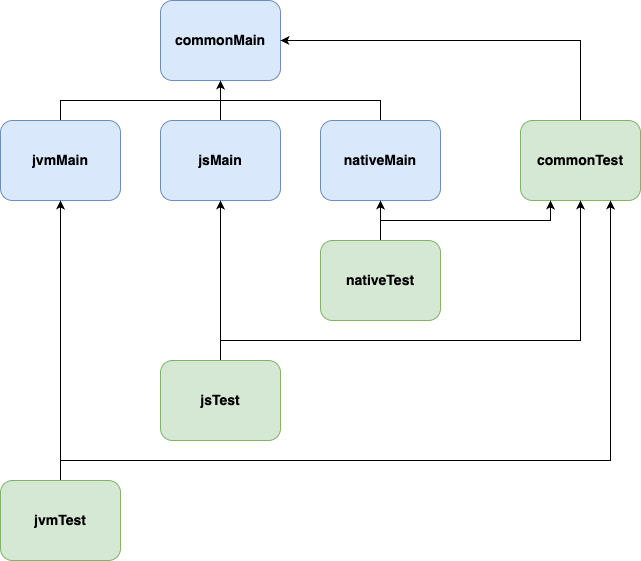
\includegraphics[width=0.95\textwidth]{charts/kmp-structure.drawio.png}
    \caption{Przykładowa struktura pojektu Kotlin Multiplatform [źródło:~opracowanie~własne]}
    \label{fig:kmp_project_structure}
\end{figure}

Następnie programista może utworzyć kolejne katalogi, które będą zawierać kod specyficzny dla docelowych platform.
Przykładowa struktura została przedstawiona na Rysunku \ref{fig:kmp_project_structure}, gdzie katalog commonMain jest wspóldzielony między JVM (jvmMain), JavaScript (jsMain) oraz platformy natywne (nativeMain).
Docelowe platformy (ang. targets) są deklarowane w konfiguracji Gradle \cite{kotlinMultiplatformDev}, a kod współdzielony jest przygotowywany wyłącznie dla nich.
Katalogi dla docelowych platform są wymagane, gdyż Kotlin nie zezwala na użycie specyficznych elementów danej platformy w katalogu współdzielonym.
Przykładem takiego elementu może być klasa ,,java.io.File'', która jest dostępna wyłącznie dla maszyny wirtualnej Javy.
Jej użycie w katalogu commonMain spowoduje błąd kompilacji.

Kotlin Multiplatform zawiera także integracje z testami oprogramowania.
Jest to szczególnie ważne dla tworzenia oprogramowania z wykorzystaniem AWS Lambda, gdzie testowanie może być skomplikowane (co było jednym z wniosków przeglądu literatury w Rozdziale \ref{chapter:przeglad_literatury}).
Testy dla kodu współdzielonego powinny być zapisane w katalogu ,,commonTest'', gdzie programista może użyć biblioteki kotlin.test \cite{kotlinMultiplatformDev}.
Następnie testy są uruchamiane dla każdej docelowej platformy.
Programista może także tworzyć przypadki testowe dla konkretnych platform, z użyciem technologii przez nie oferowanych.
Następuje tutaj analogiczne współdzielenie kodu jak dla katalogów ,,main'', co zostało także zawarte w Rysunku \ref{fig:kmp_project_structure}.

Specyficzne cechy Kotlina jak funkcjonalności języka, biblioteki czy projekt Kotlin Multiplatform mogą zapewnić znaczne wzrosty wydajności funkcji AWS Lambda.
Mimo, że Kotlin jest językiem wywodzącym się z Javy oferuje już możliwości, które mogą pozwolić na osiągnięcie niższych czasów odpowiedzi.
Dodatkowo, sposoby te nie zostały jeszcze przebadane. 
Dlatego Kotlin to obszar, który zasługuje na zawarcie go w badanich na temat wydajności AWS Lambda.
